Sono stati effettuati un totale di 241 lanci di dadi. 

\begin{table}[H]
	\centering
	\begin{tabular}{|c|c|}
		\hline
		\textbf{Valore} & \textbf{Frequenza Assoluta} \\
		\hline
		11 & 17 \\
		\hline
		8 & 17 \\
		\hline
		6 & 17 \\
		\hline
		7 & 16 \\
		\hline
		12 & 16 \\
		\hline
		5 & 16 \\
		\hline
		14 & 15 \\
		\hline
		17 & 15 \\
		\hline
		19 & 14 \\
		\hline
		10 & 12 \\
		\hline
		18 & 11 \\
		\hline
		4 & 10 \\
		\hline
		13 & 9 \\
		\hline
		15 & 9 \\
		\hline
		9 & 8 \\
		\hline
		16 & 8 \\
		\hline
		3 & 7 \\
		\hline
		20 & 7 \\
		\hline
		21 & 6 \\
		\hline
		22 & 6 \\
		\hline
		2 & 2 \\
		\hline
		23 & 2 \\
		\hline
		24 & 1 \\
		\hline
	\end{tabular}
	\caption{Tabella delle frequenze assolute della somma dei punteggi ottenuti nel lancio dei due dadi.}
	\label{tab:frequenze_assolute}
\end{table}


I dati riportati in Tabella 1 sono stati raccolti in un istogramma normalizzato.

\begin{figure}[H]
	\centering
	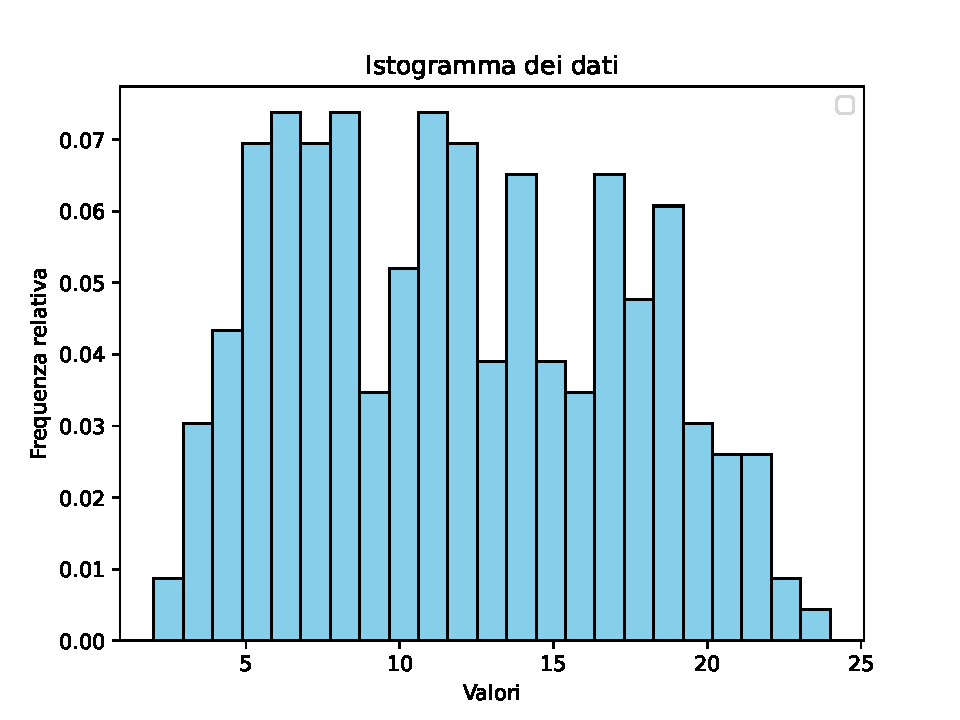
\includegraphics[width=1\textwidth]{istogramma2.pdf}
	\caption{L'istogramma comprende un totale di $N=241$ campioni in $k=23$ bins nell'intervallo $[2,\ 24]$}
\end{figure}
